\documentclass{beamer}

\usefonttheme{professionalfonts} % using non standard fonts for beamer
\usefonttheme{serif} % default family is serif

\usepackage{hyperref}
%\usepackage{minted}
\usepackage{animate}
\usepackage{graphicx}
\def\Put(#1,#2)#3{\leavevmode\makebox(0,0){\put(#1,#2){#3}}}
\usepackage{colortbl}
\usepackage{tikz}
\usepackage{amssymb}
\usepackage{enumerate}
\usepackage{arydshln}
\usepackage{algorithm}
\usepackage{algpseudocode}

\colorlet{lightred}{red!25}
\colorlet{lightgreen}{green!25}


\newcommand\blfootnote[1]{%

  \begingroup

  \renewcommand\thefootnote{}\footnote{#1}%

  \addtocounter{footnote}{-1}%

  \endgroup

}

\makeatletter

%%%%%%%%%%%%%%%%%%%%%%%%%%%%%% Textclass specific LaTeX commands.

 % this default might be overridden by plain title style

 \newcommand\makebeamertitle{\frame{\maketitle}}%

 % (ERT) argument for the TOC

 \AtBeginDocument{%

   \let\origtableofcontents=\tableofcontents

   \def\tableofcontents{\@ifnextchar[{\origtableofcontents}{\gobbletableofcontents}}

   \def\gobbletableofcontents#1{\origtableofcontents}

 }

%%%%%%%%%%%%%%%%%%%%%%%%%%%%%% User specified LaTeX commands.

\usetheme{Malmoe}

% or ...

\useoutertheme{infolines}

\addtobeamertemplate{headline}{}{\vskip2pt}

\setbeamercovered{transparent}

% or whatever (possibly just delete it)

\makeatother

\begin{document}
\title[PFLOCK report]{PFLOCK Report}
\author[AC]{Andres Calderon}
\institute[Fall'19]{University of California, Riverside}
\makebeamertitle
\newif\iflattersubsect

\AtBeginSection[] {
    \begin{frame}<beamer>
    \frametitle{Outline} 
    \tableofcontents[currentsection]  
    \end{frame}
    \lattersubsectfalse
}

\AtBeginSubsection[] {
    \begin{frame}<beamer>
    \frametitle{Outline} 
    \tableofcontents[currentsubsection]  
    \end{frame}
}

\begin{frame}{Task analysis...}
    \begin{itemize}
        \item Apache Spark divides the work into a number of Stages, each one is also divide into a number of Tasks.
        \item Each Task evaluates the data from a particular Partition and it is sent to an Executor for evaluation.
        \item Tracking the Tasks will give us a notion of the Partitions and Executors performance...
    \end{itemize}
\end{frame}

\begin{frame}{Task analysis...}
    \begin{itemize}
        \item SparkListener class allows us to monitor Taks metrics.  We can capture info about:
        \begin{itemize}
            \item executor: The id of the executor where the Task was evaluated.
            \item duration: Execution time of the task.
            \item recordsRead/Written: Total number of records read or written.
            \item bytesRead/Written: Total number of bytes read or written.
            \item shuffleRead/Written: Total number of records read or written from the shuffle by this task.
        \end{itemize}
    \end{itemize}
\end{frame}

\begin{frame}{Task analysis...}
    \begin{itemize}
        \item Running experiments with Epsilon=30, Mu=3 and Delta=3.
        \item Collecting Task metrics.  Focus on Time by time implementation...
    \end{itemize}
    \begin{figure}
        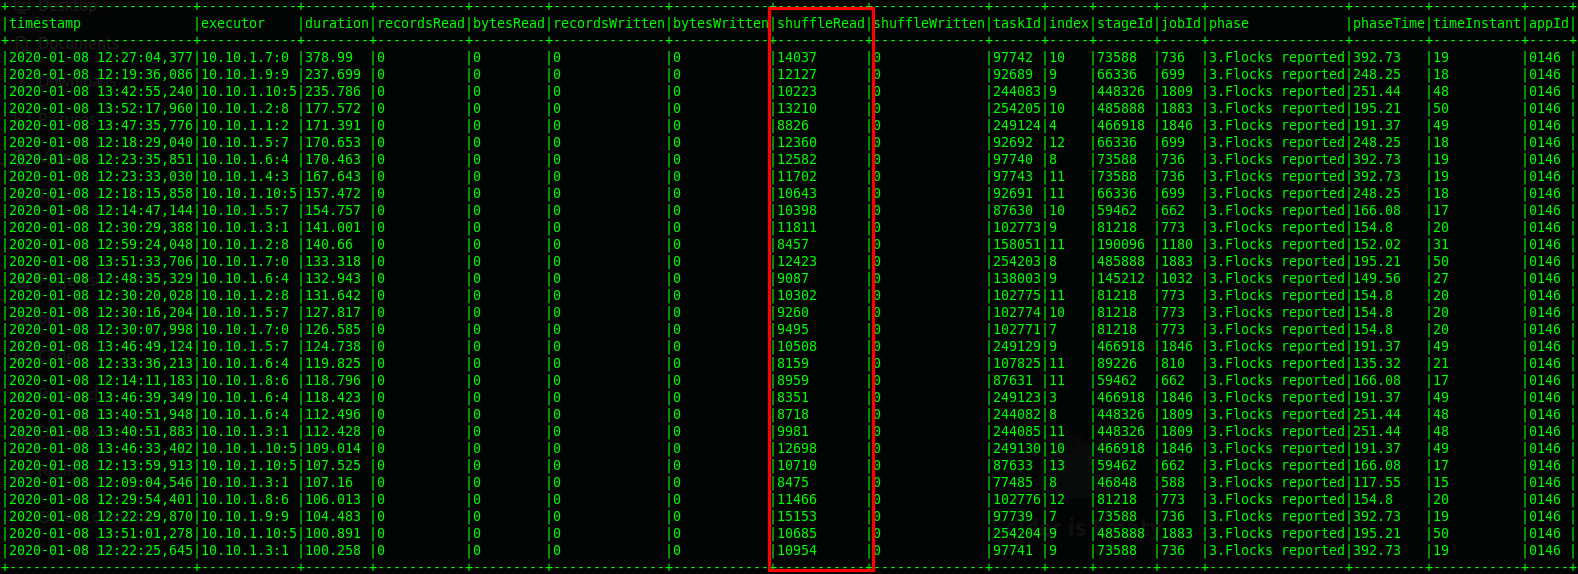
\includegraphics[width=1\textwidth]{figures/TaskAnalysisFF1}
        \caption{\small Top 30 longest tasks}
    \end{figure}
\end{frame}

\begin{frame}{Task analysis...}
    \begin{itemize}
        \item Running experiments with Epsilon=30, Mu=3 and Delta=3.
        \item Collecting Task metrics.  Focus on Time by time implementation...
    \end{itemize}
    \begin{figure}
        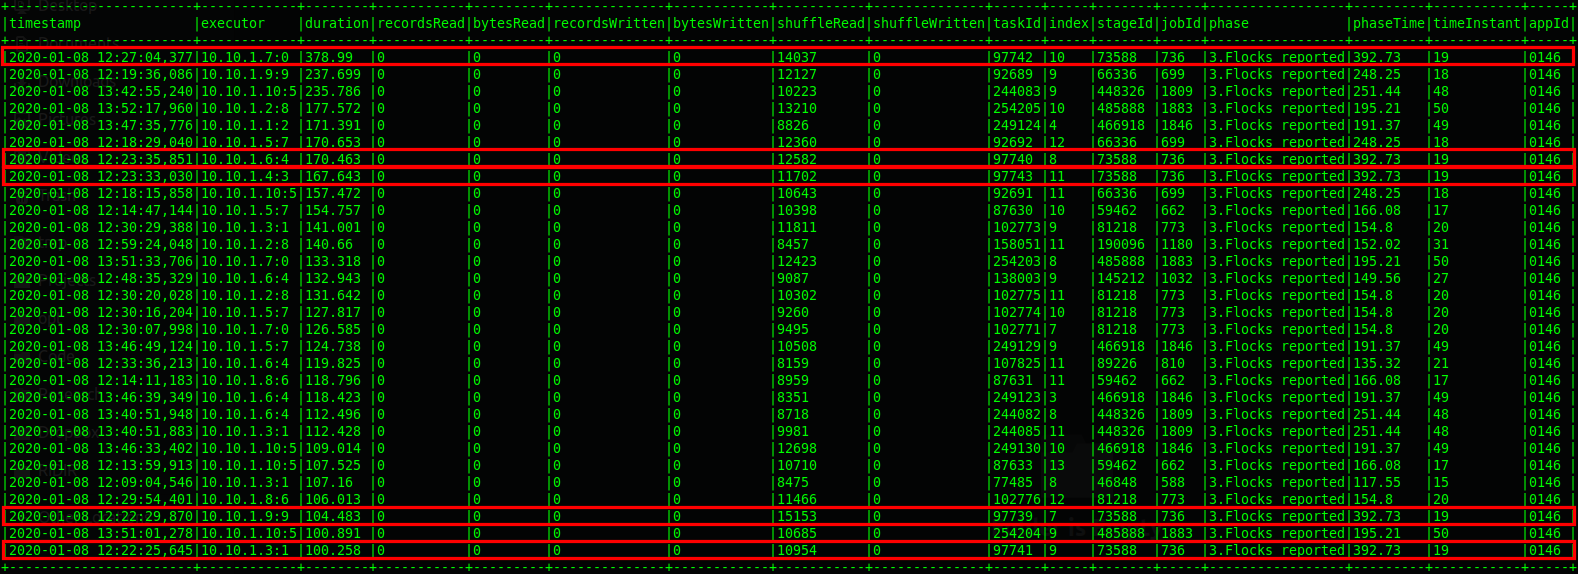
\includegraphics[width=1\textwidth]{figures/TaskAnalysisFF2}
        \caption{\small Top 30 longest tasks}
    \end{figure}
\end{frame}

\begin{frame}{Stage analysis...}
    \begin{itemize}
        \item SparkListener also provide info about the whole stage.  Some interesting metrics are:
        \begin{itemize}
            \item numTasks: The number of tasks in which the Stage is divided.
            \item name: The Spark function which invoke the Stage and its line of code.
            \item details: The stack trace when the Stage was called.
        \end{itemize}
    \end{itemize}

    \begin{figure}
        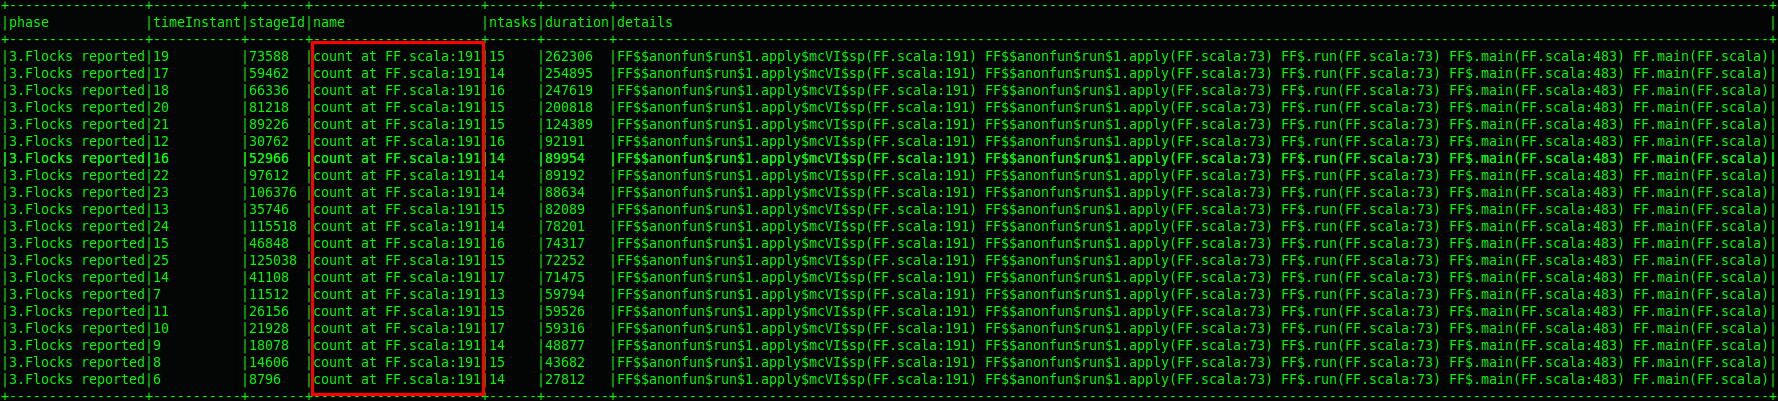
\includegraphics[width=1\textwidth]{figures/StageAnalysisFF1}
        \caption{\small Top 20 longest stages}
    \end{figure}
\end{frame}

\begin{frame}{Stage analysis...}
    \begin{itemize}
        \item FF.scala:191 makes a call to the redundant flocks prunning routine.
        \item I have noted that I am repartitioning the data in order to match the prevoius set of flocks which could be causing the shuffling.
        \item Currently I have extracted some data for testing (time instant 19) and making some improvements.
    \end{itemize}
\end{frame}

\begin{frame}{What is next...}
    \begin{itemize}
        \item Fixi the shuffling overheard during the prunning routine.
        \item Perform similar analysis for the Time window implementation.
    \end{itemize}
\end{frame}

\end{document}
